
\addtocounter{framenumber}{-8}

\begin{frame}
\frametitle{Our Agenda}
\large 

\begin{columns}[t]
	\column{.5\textwidth}
	use pure \textbf<1>{data-driven end-to-end} learning
	\begin{itemize}
		\item no pre/postprocessing of data
		\item top-of-atmosphere data
		\item no atmospheric correction
		\item no cloud filtering
		\item no additional image registration
	\end{itemize}
	\vspace{1em}
	adapt established methods to EO Sensors
	\begin{itemize}
		\item NLP to EO: Sentence translation to image sequence classification
	\end{itemize}
	
	\column{.5\textwidth}
	\vspace{-2em}
	\uncover<1->{
		\centering 
		
\tikzsetnextfilename{datenbasiert}

% exclude this file from externalize otherwise the if else condition dies not work
\tikzset{external/export=false}
\begin{tikzpicture}[]

% if drawdl the deep learning part is drawn
\providecommand{\drawdl}{1}

\def\size{1.5cm}
\def\iosize{1.5cm}

\tikzstyle{illustration}=[yshift=-5mm]
\tikzstyle{element}=[draw=tumivory, fill=white, inner sep=2mm, rounded corners, node distance=4em and 2em]
\tikzstyle{ioelement}=[draw=tumivory, fill=tumwhite, inner sep=2mm, rounded corners, node distance=4em and 2em]
\tikzstyle{edge}=[rounded corners=3mm]

\node[ioelement, align=center,label=above:{$\M{X}$}](input){\resizebox{\iosize}{!}{\begin{tikzpicture}
	% each layer
	
	% raster size
  \def\d{0.73}  	
	
	% distance layer
	\def\s{\d*5}
	
	\foreach \i in {1,...,6}
	{		
		\begin{scope}[
      yshift=\s*\i,every node/.append style={
			yslant=0.5,xslant=-1},yslant=0.5,xslant=-1
		]
		%\draw[step=3.33mm] (0,0) grid (1,1);
		%\fill[black,fill opacity=.9] (0.333,0.333) rectangle (0.333,0.333);    	    	  
		
		\foreach \row in {0,...,2}{
			\foreach \col in {0,...,2}{
				\draw[tumblack, fill=tumblue!\pdfuniformdeviate 40,fill opacity=1,rounded corners=1] (\col*\d/3,\row*\d/3) rectangle (\col*\d/3+\d/3, \row*\d/3+\d/3);
	        }
		}
		\end{scope}
	}	
\end{tikzpicture}}}; %input\\$\VInput \in \R^D$
%\node[illustration,above=of input](raster){};

\node[element, right = of input,label=below:{end-to-end learning}](eelearning){
	\hspace{-1em}\def\layersep{5mm}
\def\ninput{2}
\def\nhiddenone{3}
%\def\nhiddentwo{3}
%\def\nhiddenthree{3}
\def\noutput{2}

\begin{tikzpicture}[shorten >=1pt,->,draw=black!50, node distance=\layersep, xscale=1.5, yscale=.5]
    \tikzstyle{every pin edge}=[<-,shorten <=1pt]
    \tikzstyle{neuron}=[circle,fill=black!25,minimum size=10pt,inner sep=0pt]
    \tikzstyle{input neuron}=[neuron, fill=tumbluelight];
    \tikzstyle{output neuron}=[neuron, fill=tumgray];
    \tikzstyle{hidden neuron}=[neuron, fill=tumblue];
    \tikzstyle{annot} = [text width=4em, text centered]
    % Draw the input layer nodes
    \foreach \name / \y in {1,...,\ninput}
    % This is the same as writing \foreach \name / \y in {1/1,2/2,3/3,4/4}
        \node[input neuron] (I-\name) at (0,-\y) {};
        
    % Draw the hidden layer nodes
    \foreach \name / \y in {1,...,\nhiddenone}
        \path[yshift=0.5cm]
            node[hidden neuron] (Hone-\name) at (\layersep,-\y cm) {};
%            
%    % Draw the hidden layer nodes
%    \foreach \name / \y in {1,...,\nhiddentwo}
%        \path[yshift=0.5cm]
%        node[hidden neuron] (Htwo-\name) at (2*\layersep,-\y cm) {};
%        
%    % Draw the hidden layer nodes
%    \foreach \name / \y in {1,...,\nhiddenthree}
%       \path[yshift=0.5cm]
%        node[hidden neuron] (Hthree-\name) at (3*\layersep,-\y cm) {};
%                
	\foreach \name / \y in {1,...,\noutput}
	 % This is the same as writing \foreach \name / \y in {1/1,2/2,3/3,4/4}
	 \node[output neuron] (O-\name) at (2*\layersep,-\y) {};

    % Draw the output layer nodem
%    \node[output neuron,pin={[pin edge={->}]right:Output}, right of=Htwo-2] (O) {};

    % Connect every node in the input layer with every node in the
    % hidden layer.
    \foreach \source in {1,...,\ninput}
        \foreach \dest in {1,...,\nhiddenone}
            \path (I-\source) edge (Hone-\dest);
%            
%    \foreach \source in {1,...,\nhiddenone}
%       \foreach \dest in {1,...,\nhiddentwo}
%        \path (Hone-\source) edge (Htwo-\dest);
%        
%   \foreach \source in {1,...,\nhiddentwo}
%      \foreach \dest in {1,...,\nhiddenthree}
%        \path (Htwo-\source) edge (Hthree-\dest);
        
    \foreach \source in {1,...,\nhiddenone}
      \foreach \dest in {1,...,\noutput}
        \path (Hone-\source) edge (O-\dest);

    % Connect every node in the hidden layer with the output layer
%    \foreach \source in {1,...,\nhiddenone}
%        \path (Htwo-\source) edge (O);

    % Annotate the layers
%    \node[annot,above of=H-1, node distance=1cm] (hl) {Hidden layer};
%    \node[annot,above of=I-1] {$\VInput$};
%    \node[annot,above of=O-1] {$\V{y}$};
\end{tikzpicture}
}; %\emph{end-to-end learning}

\node[ioelement,right=of eelearning, align=center,label=above:{$\V{y}$}](result){
	\resizebox{!}{\iosize}{
%		\rotatebox{90}{
			\tikz{
	\begin{scope}[rotate=90]
	%\draw[step=0.2] (0,0) grid (2,.2);
	\foreach \i in {0,...,6}
	\draw[tumblack,fill=tumorange!\pdfuniformdeviate 40,fill opacity=.9, rounded corners=0.5] (\i*.2,0) rectangle (\i*.2+.2,.2);
	%       \draw[black,fill=black!\pdfuniformdeviate 40,fill opacity=.9, rounded corners=0.5] (\i*.2,0) rectangle (\i*.2+.2,.2);
	
	\end{scope}
}
%		}
	}
};
%\node[illustration,above=of result](classprob){\resizebox{1cm}{!}{\vectorgrid}};


% arrows
\draw [-stealth, edge, draw=black] (input) -- (eelearning) -- (result);


\end{tikzpicture}

	}
	
	%			\vspace{1em}
	
	
\end{columns}

\end{frame}


\begin{frame}{UCR Datasets}

%	\begin{columns}
%		\column{.6\textwidth}
%		
\begin{itemize}[leftmargin=0cm]
	\item broad family of \textbf{46 diverse datasets}
	\item \textbf{accuracies reported} from other early classification approaches
	\item covers \textbf{sensor data}, \textbf{motion tracking}, \textbf{electrocardiography data}
	\item many, but \textbf{small datasets} \small{(overall circa 500 MB)}
\end{itemize}
%		\column{.4\textwidth}
%		\includegraphics[width=\textwidth]{images/UCR}
%	\end{columns}

\vspace{.5em}
\centering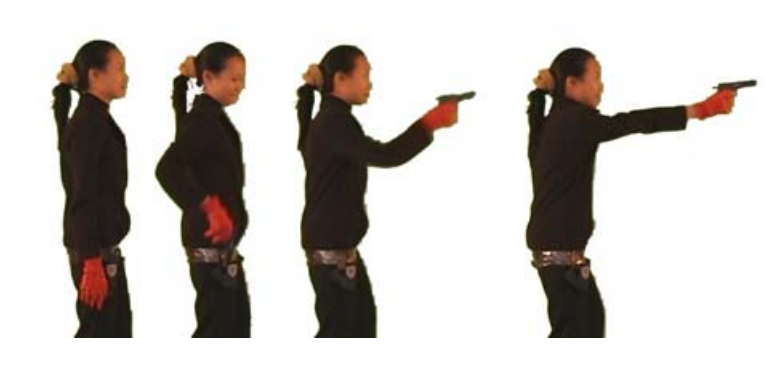
\includegraphics[width=5cm]{images/GunPoint}

\vspace{.5em}

{\small \texttt{http://www.timeseriesclassification.com/}
}
\end{frame}


\begin{frame}
\frametitle{Communications}
\centering
\begin{tikzpicture}[xscale=3.5, yscale=2]
%\draw[fill=tumblue, draw=none, opacity=0.5](-1,0) circle (1.5);
\node[fill=tumbluelight, draw=none, opacity=0.5, circle, minimum width=6cm, label=Earth Observation] at (-1,0){};

\node[fill=tumorange!50, draw=none, opacity=0.5, circle, minimum width=6cm, label=Machine Learning] at (1,0){};
%\draw[fill=tumorange, draw=none, opacity=0.5](1,0) circle (1.5);

%\node at (-1.3,1){Data};

\node[text width=3.5cm] at (-1,.9){\focusmethod is a \textbf{tool} for our \focusdata};
\node[text width=3.5cm] at (1,.9){\focusdata is a \textbf{benchmark} for our \focusmethod};


\node[text width=3.5cm] at (-1,.3){\textbf{should generalize} to applications of a \\ specific sub-field};
\node[text width=3.5cm] at (1,.3){\textbf{must generalize} to many fields of applications};

\node[text width=3.5cm] at (-1,-.3){data has specific \\ \textbf{phyisical properties}};
\node[text width=3.5cm] at (1,-.3){data is a \textbf{feature vector}};
%
%\node[text width=2cm] at (-1.3,-.6){{physics}, {sensors}, {applications}};

%\node at (1.3,1){Method};

%\node at (-1.3,1){IGARSS};
%\node at (-1.6,-1){ISPRS};
%\node at (-1.2,-.6){IEEE-GRSS};
%\node at (-1.8,.4){MDPI-RS Journal};
%\node at (-1.3,0){RSE Journal};
%
%\node at (1.3,1){NeurIPS};
%\node at (1.6,-1){CVPR};
%\node at (1.2,-.6){ICML};
%\node at (1.8,.4){ECCV};
%\node at (1.3,.2){ECML};
%
%\node at (0,.5){CVPR EarthVision};
%\node at (0,0){ECML MACLEAN};
%\node at (0,-.5){(ESA-$\Phi$-week)};

\end{tikzpicture}

\end{frame}

\begin{frame}<presentation:3>
\frametitle{Chair of Remote Sensing Technology}


    \resizebox{\linewidth}{!}{
      \begin{tikzpicture}[scale=.75,font=\scriptsize,draw=tumblue]
        
        % university
        \draw[draw,fill=tumbluelight] (0,0) rectangle node{Technical University of Munich} +(9, 1);
        \draw[draw=none,fill=none] (0.25,.01) rectangle node{
\includegraphics[width=1cm]{images/logo-blue-TUM.pdf}} +(1,1);
        
        % faculty
        \draw[draw] (0,1) rectangle node{} +(1,1);
        \draw[draw=none] (1,1) rectangle node{\ldots} +(1,1);
        \draw[draw, fill=tumbluelight!75] (2,1) rectangle node[align=center]{Faculty of Geo, Civil and\\ Environmental Engineering} +(7,1);

        % groups
        \draw[draw] (2,2) rectangle node{} +(1,3);
        \draw[draw=none] (3,2) rectangle node{\ldots} +(1,3);

        \draw[draw] (4,5) rectangle node[align=center, font=\tiny]{Prof.\\U. Stilla} +(1.5,1);
        \draw[draw] (4,2) rectangle node[align=center, anchor=base, yshift=-1mm, font=\tiny]{\emph{FPF}\\[1mm]Photo-\\grammetry\\and Remote\\Sensing} +(1.5,3);
        
        \visible<5->{%
          \draw[draw, fill=tumbluelight!25] (5.5,5) rectangle node[align=center, font=\tiny, name=SiPEO_XZ]{Prof.\\X. Zhu} +(1.5,1);
          \draw[draw, fill=tumbluelight!25] (5.5,2) rectangle node[align=center, anchor=base, yshift=-1mm, font=\tiny]{%
            \emph{SiPEO}\\[1mm]Signal\\Processing\\in Earth\\Observation
          } +(1.5,3);
        }
        
        \visible<2->{%
          \draw[draw, fill=tumbluelight!50] (7,5) rectangle node[align=center, font=\scriptsize\bf, name=LMF_RB] {Prof.\\R. Bamler} +(2,1);
          \draw[draw, fill=tumbluelight!50] (7,2) rectangle node[align=center, anchor=base, yshift=-1mm, font=\tiny]{%
            \emph{LMF}\\[1mm]Chair of \\Remote\\Sensing\\Technology
          } +(2,3);
        }

        
        \visible<3->{%
          \draw[draw=tumgreen, fill=tumgreen!50, rounded corners=3pt] (7.1,2.1) rectangle node[align=center, font=\tiny]{Computer Vision\\Research Group\\[1mm]Dr. M. Körner} +(1.8,1);
        }


        \visible<4->{%
          \draw[draw=tumorange, fill=tumorange!50] (10,1) rectangle node[align=center]{Remote Sensing Technology Institute \textit{(IMF)}} +(7.5,1);
          \draw[draw=none] (17.25,1) rectangle node{\ldots} +(1,1);
          \draw[draw=tumorange] (18,1) rectangle node{} +(1,1);

          \draw[draw=tumorange, fill=tumorange!75] (10,0) rectangle node[align=center]{German Aerospace Center\\Campus Oberpfaffenhofen near Munich} +(9, 1);
          \draw[draw=none,fill=none] (17.5,.01) rectangle node{
\includegraphics[height=.6cm]{images/logo-black-DLR}} +(1,1);

          \draw[draw=tumorange, fill=tumorange!25] (10,2) rectangle node[align=center, font=\tiny]{Photo-\\grammetry\\ and\\Image\\Analysis} +(1.5,2);
          \draw[draw=tumorange, fill=tumorange!25] (10,4) rectangle node[align=center, font=\tiny]{Prof.\\P. Reinartz} +(1.5,1);

          \draw[draw=tumorange, fill=tumorange!25] (11.5,2) rectangle node[align=center, font=\tiny]{SAR\\Signal\\Processing} +(1.5,2);
          \draw[draw=tumorange, fill=tumorange!25] (11.5,4) rectangle node[align=center, font=\tiny]{Prof.\\M. Eineder} +(1.5,1);

          \draw[draw=tumorange, fill=tumorange!25] (13.0,2) rectangle node[align=center, font=\tiny]{Atmospheric\\ Processors} +(1.5,2);
          \draw[draw=tumorange, fill=tumorange!25] (13.0,4) rectangle node[align=center, font=\tiny]{Prof.\\T. Trautmann} +(1.5,1);

          \draw[draw=tumorange, fill=tumorange!25] (14.50,2) rectangle node[align=center, font=\tiny]{Experimental\\ Methods} +(1.5,2);
          \draw[draw=tumorange, fill=tumorange!25] (14.50,4) rectangle node[align=center, font=\tiny]{Prof. P. \\Haschberger} +(1.5,1);

%          \visible<5->{%
            \draw[draw=tumorange, fill=tumorange!25] (16.00,2) rectangle node[align=center, font=\tiny]{Data Science\\ in Earth\\ Observation} +(1.5,2);
            \draw[draw=tumorange, fill=tumorange!25] (16.00,4) rectangle node[align=center, font=\tiny, name=DAS_XZ]{Prof.\\ X. Zhu} +(1.5,1);
%          }

          \draw[draw=tumorange, fill=tumorange!25] (10,5) rectangle node[align=center, font=\scriptsize\bf]{Prof. R. Bamler} +(7.5,1) ;


        %   \draw[draw=none, shade, left color=tumbluelight, right color=tumorange!25] (9,2) rectangle node{} +(1,4);
          \fill[draw=none, draw opacity=0, shade, left color=tumbluelight!50, right color=tumorange!25] (9,2) -- (9,6) -- (10,6) -- (10,1) -- cycle;
          \draw[stealth-stealth] (9,5.5) -- (10,5.5) ;
        
%           \draw[stealth-stealth] (SiPEO_XZ.north) |- +(0,1) -| (DAS_XZ.north) +(-1,0);
        }

      \end{tikzpicture}
    }
\end{frame}

\begin{frame}<presentation:5>
\frametitle{Chair of Remote Sensing Technology}


    \resizebox{\linewidth}{!}{
      \begin{tikzpicture}[scale=.75,font=\scriptsize,draw=tumblue]
        
        % university
        \draw[draw,fill=tumbluelight] (0,0) rectangle node{Technical University of Munich} +(9, 1);
        \draw[draw=none,fill=none] (0.25,.01) rectangle node{
\includegraphics[width=1cm]{images/logo-blue-TUM.pdf}} +(1,1);
        
        % faculty
        \draw[draw] (0,1) rectangle node{} +(1,1);
        \draw[draw=none] (1,1) rectangle node{\ldots} +(1,1);
        \draw[draw, fill=tumbluelight!75] (2,1) rectangle node[align=center]{Faculty of Geo, Civil and\\ Environmental Engineering} +(7,1);

        % groups
        \draw[draw] (2,2) rectangle node{} +(1,3);
        \draw[draw=none] (3,2) rectangle node{\ldots} +(1,3);

        \draw[draw] (4,5) rectangle node[align=center, font=\tiny]{Prof.\\U. Stilla} +(1.5,1);
        \draw[draw] (4,2) rectangle node[align=center, anchor=base, yshift=-1mm, font=\tiny]{\emph{FPF}\\[1mm]Photo-\\grammetry\\and Remote\\Sensing} +(1.5,3);
        
        \visible<5->{%
          \draw[draw, fill=tumbluelight!25] (5.5,5) rectangle node[align=center, font=\tiny, name=SiPEO_XZ]{Prof.\\X. Zhu} +(1.5,1);
          \draw[draw, fill=tumbluelight!25] (5.5,2) rectangle node[align=center, anchor=base, yshift=-1mm, font=\tiny]{%
            \emph{SiPEO}\\[1mm]Signal\\Processing\\in Earth\\Observation
          } +(1.5,3);
        }
        
        \visible<2->{%
          \draw[draw, fill=tumbluelight!50] (7,5) rectangle node[align=center, font=\scriptsize\bf, name=LMF_RB] {Prof.\\R. Bamler} +(2,1);
          \draw[draw, fill=tumbluelight!50] (7,2) rectangle node[align=center, anchor=base, yshift=-1mm, font=\tiny]{%
            \emph{LMF}\\[1mm]Chair of \\Remote\\Sensing\\Technology
          } +(2,3);
        }

        
        \visible<3->{%
          \draw[draw=tumgreen, fill=tumgreen!50, rounded corners=3pt] (7.1,2.1) rectangle node[align=center, font=\tiny]{Computer Vision\\Research Group\\[1mm]Dr. M. Körner} +(1.8,1);
        }


        \visible<4->{%
          \draw[draw=tumorange, fill=tumorange!50] (10,1) rectangle node[align=center]{Remote Sensing Technology Institute \textit{(IMF)}} +(7.5,1);
          \draw[draw=none] (17.25,1) rectangle node{\ldots} +(1,1);
          \draw[draw=tumorange] (18,1) rectangle node{} +(1,1);

          \draw[draw=tumorange, fill=tumorange!75] (10,0) rectangle node[align=center]{German Aerospace Center\\Campus Oberpfaffenhofen near Munich} +(9, 1);
          \draw[draw=none,fill=none] (17.5,.01) rectangle node{
\includegraphics[height=.6cm]{images/logo-black-DLR}} +(1,1);

          \draw[draw=tumorange, fill=tumorange!25] (10,2) rectangle node[align=center, font=\tiny]{Photo-\\grammetry\\ and\\Image\\Analysis} +(1.5,2);
          \draw[draw=tumorange, fill=tumorange!25] (10,4) rectangle node[align=center, font=\tiny]{Prof.\\P. Reinartz} +(1.5,1);

          \draw[draw=tumorange, fill=tumorange!25] (11.5,2) rectangle node[align=center, font=\tiny]{SAR\\Signal\\Processing} +(1.5,2);
          \draw[draw=tumorange, fill=tumorange!25] (11.5,4) rectangle node[align=center, font=\tiny]{Prof.\\M. Eineder} +(1.5,1);

          \draw[draw=tumorange, fill=tumorange!25] (13.0,2) rectangle node[align=center, font=\tiny]{Atmospheric\\ Processors} +(1.5,2);
          \draw[draw=tumorange, fill=tumorange!25] (13.0,4) rectangle node[align=center, font=\tiny]{Prof.\\T. Trautmann} +(1.5,1);

          \draw[draw=tumorange, fill=tumorange!25] (14.50,2) rectangle node[align=center, font=\tiny]{Experimental\\ Methods} +(1.5,2);
          \draw[draw=tumorange, fill=tumorange!25] (14.50,4) rectangle node[align=center, font=\tiny]{Prof. P. \\Haschberger} +(1.5,1);

%          \visible<5->{%
            \draw[draw=tumorange, fill=tumorange!25] (16.00,2) rectangle node[align=center, font=\tiny]{Data Science\\ in Earth\\ Observation} +(1.5,2);
            \draw[draw=tumorange, fill=tumorange!25] (16.00,4) rectangle node[align=center, font=\tiny, name=DAS_XZ]{Prof.\\ X. Zhu} +(1.5,1);
%          }

          \draw[draw=tumorange, fill=tumorange!25] (10,5) rectangle node[align=center, font=\scriptsize\bf]{Prof. R. Bamler} +(7.5,1) ;


        %   \draw[draw=none, shade, left color=tumbluelight, right color=tumorange!25] (9,2) rectangle node{} +(1,4);
          \fill[draw=none, draw opacity=0, shade, left color=tumbluelight!50, right color=tumorange!25] (9,2) -- (9,6) -- (10,6) -- (10,1) -- cycle;
          \draw[stealth-stealth] (9,5.5) -- (10,5.5) ;
        
%           \draw[stealth-stealth] (SiPEO_XZ.north) |- +(0,1) -| (DAS_XZ.north) +(-1,0);
        }

      \end{tikzpicture}
    }
\end{frame}


\begin{frame}
\frametitle{Summary: Balancing Resolutions}

\begin{columns}
	\column{.5\textwidth}


\begin{tikzpicture}[scale=3,
x={(\raarot cm,\rbarot cm)},%
y={(\rabrot cm, \rbbrot cm)},%
z={(\racrot cm, \rbcrot cm)}]




\draw [->] (0,0,0) -- (1.2,0,0) node[anchor=north east]{spatial};
\draw [->] (0,0,0) -- (0,1.2,0) node[anchor=north west]{spectral};
\draw [->] (0,0,0) -- (0,0,1.2) node[anchor=south]{temporal};   

\draw (0,0,1) node[right] {hours};
\draw (0,0,0.66) node[right] {days};
\draw (0,0,0.33) node[right] {weeks};

\draw (0,.33,0) node[right] {3};
\draw (0,.66,0) node[right] {15};
\draw (0,1,0) node[right] {$>$100};

\draw (1,0,0) node[above left] {$<$1m};
\draw (.8,0,0) node[above left] {10m};
\draw (.6,0,0) node[above left] {100m};
\draw (.4,0,0) node[above left] {1km};
\draw (.2,0,0) node[above left] {10km};


%% High Resolution
\visible<2>{\domain{1.2}{0.4}{.6}{tumgreen};}

%% environmental satellites
\visible<3>{\domain{0.5}{.9}{.9}{tumorange};}

%% Hyper-spectral
\visible<4>{\domain{0.7}{1.3}{.2}{tumgreen};}

%% Multi-spectral
\visible<5>{\domain{0.9}{.7}{.7}{tumgreen};}

%% weather satellites	
\visible<6>{\domain{0.3}{.6}{1.2}{tumblue};}

\end{tikzpicture}

\column{.5\textwidth}

\visible<2->{
	\textbf{Scheduled Acquisitions}
	\begin{itemize}
		\item<2-> very high spatial Resolution Imagery
	\end{itemize}
}
\visible<3->{
	\textbf{Global coverage and open data policy}
	\begin{itemize}
		\item<3-> multi-spectral satellites
		\item<4-> environmental satellites
		\item<5-> weather satellites
	\end{itemize}
	
}

\end{columns}
\end{frame}


\begin{frame}
\frametitle{Augmenting Classification Models}

\begin{columns}
	
	\column{.5\textwidth}
	\begin{center}
		
		\begin{tikzpicture}[node distance=1em and 1.5em]
\node[](x0){$x_t$};
\node[rnn, below=of x0](h0){\small$f\left(\xuptot\right)$};
\node[below right= 2em and .0em of h0](y0){$\yhat_t$};
\node[rnn, left=2em of h0,draw=lightgray](hprev){};
\node[rnn, right=2em of h0,draw=lightgray](hnext){};

\draw[infer] (x0) -- (h0);
\draw[infer,draw=lightgray] (hprev) -- (h0);
\draw[infer,draw=lightgray] (h0) -- (hnext);
\draw[infer] (h0) -- (y0) node[midway,right, text=black](wc){$\theta_{cl}$};

\visible<2->{
\node[below left= 2em and .0em of h0](d0){$\delta_t$};
\draw[infer] (h0) -- (d0) node[midway,left, text=black](wd){$\theta_{\delta}$};
}

\visible<3->{
	\node[loss, below=of y0](L0){$\mathcal{L}_{cl}(\yhat,\V{y})$};
	%\node[right=of L0](t0){$\V{y}_t$};
	\draw[-stealth, grad] (y0) -- (L0);
	%\draw[-stealth, grad] (t0) -- (L0);
	%\draw[-stealth, grad] (L0) to [in=-25, out=25, looseness=2] node[midway, right, text=colortrain]{$\frac{\partial\mathcal{L}_{cl}}{\partial\theta_\text{rnn}}$}
	%(h0);
	
	\draw[-stealth, grad] (L0) to [bend right=30] node[near end, right, text=colortrain]{$\frac{\partial\mathcal{L}_{cl}}{\partial\theta_\text{cl}}$}
	(wc);
}

\only<4>{
\node[below=7em of h0, loss](L){$\mathcal{L}(\V{y_t},\yhat_t) = \delta_t\mathcal{L}_{cl}(\V{y_t},\yhat_t)$};
\draw[infer] (L0) -- (L);
\draw[infer] (d0) -- (L);

\draw[-stealth, grad] (L) to [bend right=30] node[midway, right, text=colortrain]{$\frac{\partial\mathcal{L}}{\partial\mathcal{L}_{cl}}$}
(L0);

\draw[-stealth, grad] (L) to [bend left=30] node[midway, left, text=colortrain]{$\frac{\partial\mathcal{L}}{\partial\theta_\delta}$}
(wd);

}

\only<5->{

\node[below=of d0](pt){$P(t)$};
\node[below=8em of h0, loss](L){$\mathcal{L}(\V{y_t},\yhat_t) = P(t)\mathcal{L}_{cl}(\V{y_t},\yhat_t)$};


\draw[infer] (L0) -- (L);
\draw[infer] (d0) -- (pt);
\draw[infer] (pt) -- (L);

%}
%
%\only<6->{
%\node[left=.5em of pt](budget){\small $\prod_{t'<t}(1-\delta_{t'})$};
%\draw[infer] (budget) -- (pt);

%\only<7->{
%	\node[left=.5em of pt](budget){$\mathcal{B}_{t-1}$};
%	
%}

\draw[-stealth, grad] (L) to [bend right=30] node[midway, right, text=colortrain]{$\frac{\partial\mathcal{L}}{\partial\mathcal{L}_{cl}}$}
(L0);

\draw[-stealth, grad] (L) to [bend left=30] node[midway, left, text=colortrain]{$\frac{\partial\mathcal{L}}{\partial P(t)}$}
(pt);

\draw[-stealth, grad] (pt) to [bend left=30] node[midway, left, text=colortrain]{$\frac{\partial P(t)}{\partial \theta_{\delta}}$}
(wd);

}

\end{tikzpicture}

	\end{center}
	\column{.5\textwidth}
	\begin{tikzpicture}

\pgfplotstableread[col sep = comma]{images/qualitative_example/early_rnn_run-sample0.csv}\mydata

\begin{groupplot}[
	group style={
		group name=my plots,
		group size=1 by 5,
		columns=1,
		xlabels at=edge bottom,
		xticklabels at=edge bottom,
		vertical sep=5pt,
	},
	ylabel near ticks,
	ylabel style={rotate=-90},
	width=\textwidth,
	height=3cm,
	axis x line=bottom,
	axis y line=left,
	enlarge x limits=0.01,
	ymajorgrids,
]

\nextgroupplot[no marks, enlarge y limits=0.05, hide x axis, ylabel={$x$}]
\addplot[thick, tumblue] table[x=t, y=x]{\mydata};

\nextgroupplot[no marks, ylabel={$\yhat_t$}, enlarge y limits=0.05, hide x axis]	
\addplot[thick,colorclassone, name path=y1] table[x=t, y=y1]{\mydata};
\addplot[thick,colorclasstwo, name path=y2] table[x=t, y=y2]{\mydata};
\addplot[thick,colorclassthree, name path=y3] table[x=t, y=y3]{\mydata};
\addplot[thick,colorclassfour, name path=y4] table[x=t, y=y4]{\mydata};

%\addplot[colorblue!20] fill between[of = y1 and axis];
%\addplot[colorhgray!20] fill between[of = y2 and axis];
%\addplot[colorgreen!20] fill between[of = y3 and axis];
%\addplot[colororange!20] fill between[of = y4 and axis];
\only<2->{
\nextgroupplot[ybar, bar width=1pt, ylabel={$\delta_t$}]
\addplot[draw=none, fill=tumblue] table[x=t, y=dt]{\mydata};
}

\only<5->{
\nextgroupplot[ybar, bar width=1pt, hide x axis, ylabel={$P(t)$}]
\addplot[draw=none, fill=tumblue] table[x=t, y=pts]{\mydata};

%\nextgroupplot[ybar, bar width=1pt, hide x axis, ylabel={$\prod_{t'<t}(1-\delta_{t'})$}]
%\addplot[draw=none, fill=tumblue, xlabel={time $t$}] table[x=t, y=Bt]{\mydata};
}

\end{groupplot}

\end{tikzpicture}

	
	
\end{columns}

\end{frame}



\begin{frame}
\frametitle{Earliness-Aware Loss function}

\Large

\begin{equation*}
\mathcal{L} = P(t)\left(\alpha (1-\yhat^+) + \left(1-\alpha\right) \frac{t}{T}\right)
\end{equation*}
\end{frame}


\begin{frame}
\frametitle{Spectral Bands}

\begin{columns}
	%	\column{.2\textwidth}
	%	
	%	\begin{equation*}
	%	\rho_{\lambda} = \int_{\lambda-\frac{b}{2}}^{\lambda-\frac{b}{2}} \rho_(\lambda) d\lambda
	%	\end{equation*}
	%	
	%	\vspace{1em}
	%	
	%	integrated between in spectral \textbf{bands} bounds $\lambda - \frac{b}{2}$ and $\lambda + \frac{b}{2}$ with the \emph{bandwidth} b.
	%	
	
	\column{.9\textwidth}
	
	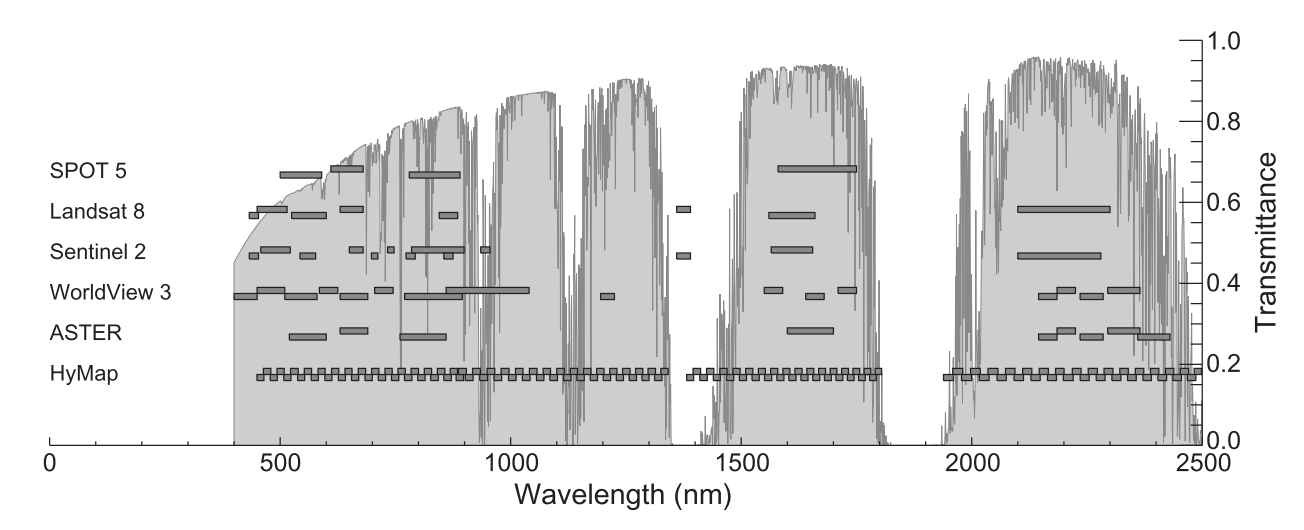
\includegraphics[width=\textwidth]{images/Meer14Satellitebands}
	
	
\end{columns}

\vspace{1em}
{\small
	Van der Meer, F. D., Van der Werff, H. M. A., \& Van Ruitenbeek, F. J. A. (2014). Potential of ESA's Sentinel-2 for geological applications. Remote sensing of environment, 148, 124-133.
}

\end{frame}


\begin{frame}{Benchmark Datasets}

%	\begin{columns}
%		\column{.6\textwidth}
%		
\begin{itemize}[leftmargin=0cm]
	\item broad family of \textbf{46 diverse datasets}
	\item \textbf{accuracies reported} from other early classification approaches
	\item covers \textbf{sensor data}, \textbf{motion tracking}, \textbf{electrocardiography data}
	\item many, but \textbf{small datasets} \small{(overall circa 500 MB)}
\end{itemize}
%		\column{.4\textwidth}
%		\includegraphics[width=\textwidth]{images/UCR}
%	\end{columns}

{\textbf{GunPoint} dataset}
\vspace{.5em}
\centering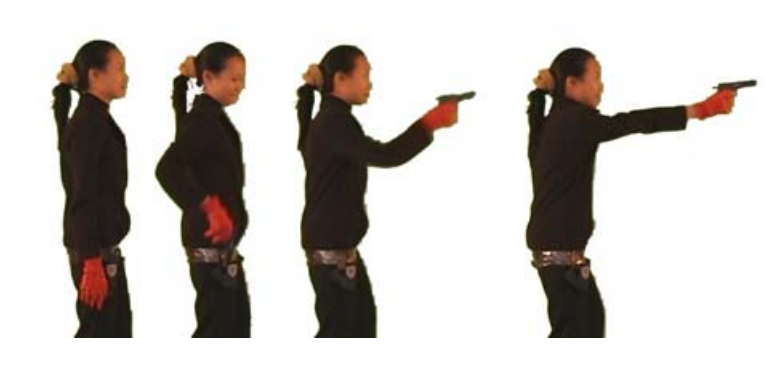
\includegraphics[width=7cm]{images/GunPoint}

\vspace{.5em}

{\small \texttt{http://www.timeseriesclassification.com/}
}
\end{frame}

\begin{frame}
\frametitle{Two Fields}
\centering
\begin{tikzpicture}[scale=2]
%\draw[fill=tumblue, draw=none, opacity=0.5](-1,0) circle (1.5);
\node[fill=tumbluelight, draw=none, opacity=0.5, circle, minimum width=6cm, label=Earth Observation] at (-1,0){};

\node[fill=tumorange!50, draw=none, opacity=0.5, circle, minimum width=6cm, label=Machine Learning] at (1,0){};
%\draw[fill=tumorange, draw=none, opacity=0.5](1,0) circle (1.5);

\draw[-stealth, shorten >=1cm] (-1.3,1) -- (0,0);
\draw[-stealth, shorten >=1cm] (-1.6,-1) -- (0,0);
\draw[-stealth, shorten >=1cm] (-1.2,-.6) -- (0,0);
\draw[-stealth, shorten >=1cm] (-1.8,.4) -- (0,0);
\draw[-stealth, shorten >=1cm] (-1.3,.2) -- (0,0);

\node[font=\bfseries] at (-2,0) {applications};

\draw[-stealth, shorten >=1cm] (1.3,1) -- (0,0);
\draw[-stealth, shorten >=1cm] (1.6,-1) -- (0,0);
\draw[-stealth, shorten >=1cm] (1.2,-.6) -- (0,0);
\draw[-stealth, shorten >=1cm] (1.8,.4) -- (0,0);
\draw[-stealth, shorten >=1cm] (1.3,.2) -- (0,0);

\node[font=\bfseries] at (2,0) {methods};

%\node[text width=2cm, circle, fill=tumblue, text=white]{global scale};
%
%\node[text width=2cm, circle, fill=tumblue, text=white]{global scale};

%\node[font=\normalsize, fill=white, text width=2cm, rounded corners, fill opacity=.5, text opacity=1](phd) at (0,0){global scaleability \\ real world impact \\ Open Data};

%\draw[-stealth, very thick] (phd) -- (0,, fil0);
\end{tikzpicture}


\end{frame}


\begin{frame}
\frametitle{Communities}
\centering
\begin{tikzpicture}[scale=2]
%\draw[fill=tumblue, draw=none, opacity=0.5](-1,0) circle (1.5);
\node[fill=tumbluelight, draw=none, opacity=0.5, circle, minimum width=6cm, label=Earth Observation] at (-1,0){};

\node[fill=tumorange!50, draw=none, opacity=0.5, circle, minimum width=6cm, label=Machine Learning] at (1,0){};
%\draw[fill=tumorange, draw=none, opacity=0.5](1,0) circle (1.5);

\node at (-1.3,1){IGARSS};
\node at (-1.6,-1){ISPRS};
\node at (-1.2,-.6){IEEE-GRSS};
\node at (-1.8,.4){MDPI-RS Journal};
\node at (-1.3,0){RSE Journal};

\node at (1.3,1){NeurIPS};
\node at (1.6,-1){CVPR};
\node at (1.2,-.6){ICML};
%\node at (1.8,.4){ECCV};
\node at (1.5,.3){AISTATS};
%\node at (1.3,.2){ECML};
\node at (1.3,-.2){ICLR};

\node at (0,.5){CVPR EarthVision};
\node at (0,0){ECML MACLEAN};
\node at (0,-.5){(ESA-$\Phi$-week)};

\end{tikzpicture}
\end{frame}


\begin{frame}
\frametitle{MODIS Satellite}
\only<1>{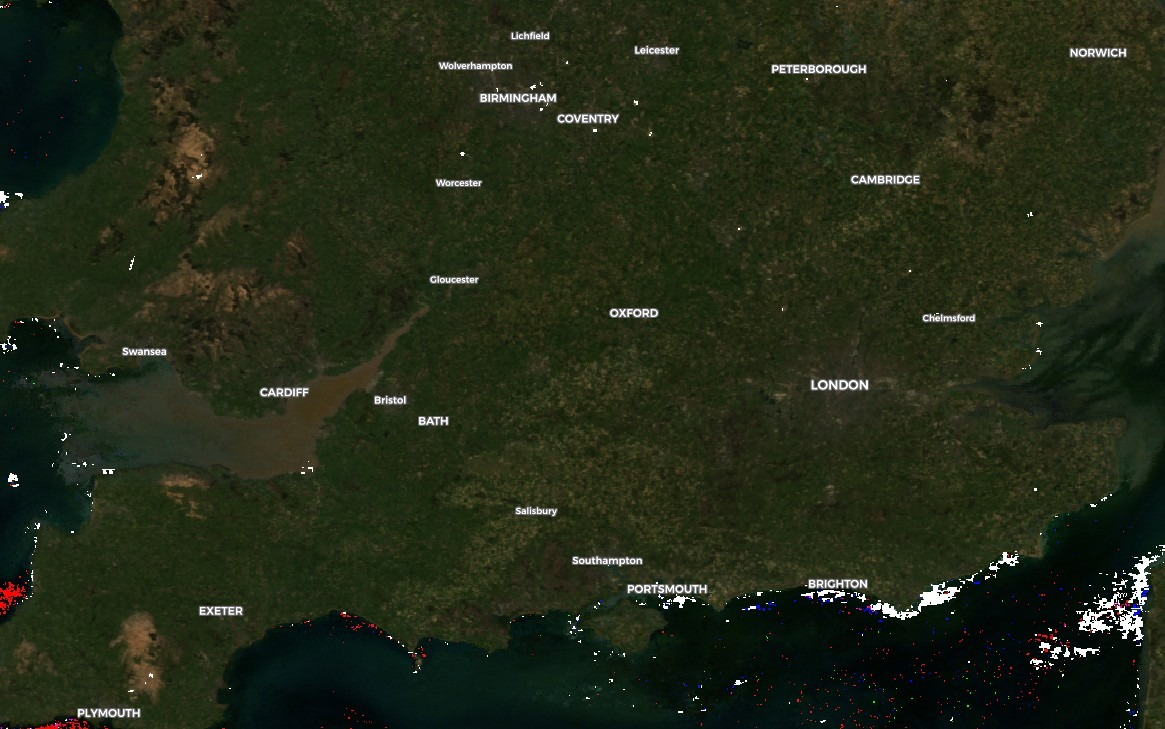
\includegraphics[width=\textwidth]{images/modis/MODIS_UK}}
\only<2>{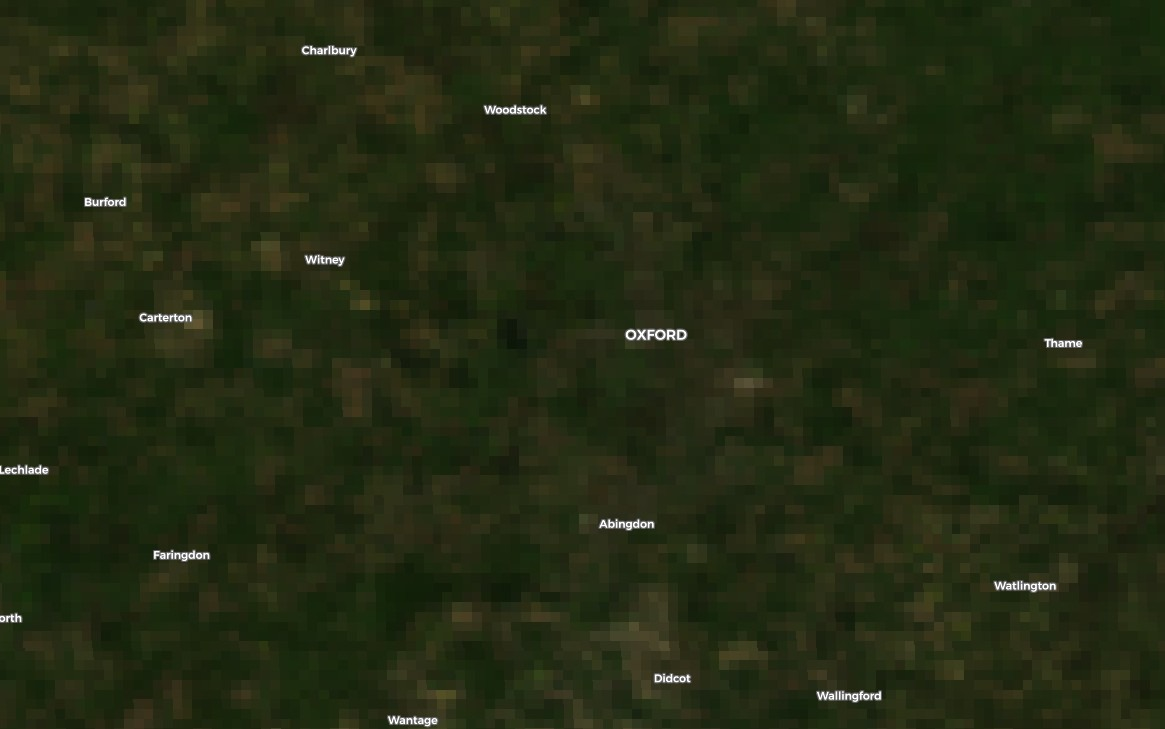
\includegraphics[width=\textwidth]{images/modis/MODIS_OXF}}
\end{frame}


